\documentclass[a4paper,11pt]{article}
\usepackage[british]{babel}
\usepackage{fullpage}
\usepackage{amsmath,amssymb}
\usepackage{multirow}
\usepackage{caption}
\usepackage{tikz,pgfplots}
\usepackage{hyperref}
\usepackage{graphicx}
\usepackage{enumitem}

\title{\textbf{Low-level Parallel Programming (course 1DL550) \\
    Uppsala University -- Spring 2015 \\
    Report for Lab 1 by Team 14}}
\author{Fredrik Larsson \and Jimmy Holm \and Per Bergqwist}
\date{\today}

\begin{document}
\maketitle

\section{Plot}
\begin{center}
  \pgfplotsset{grid style={dotted,gray}}
  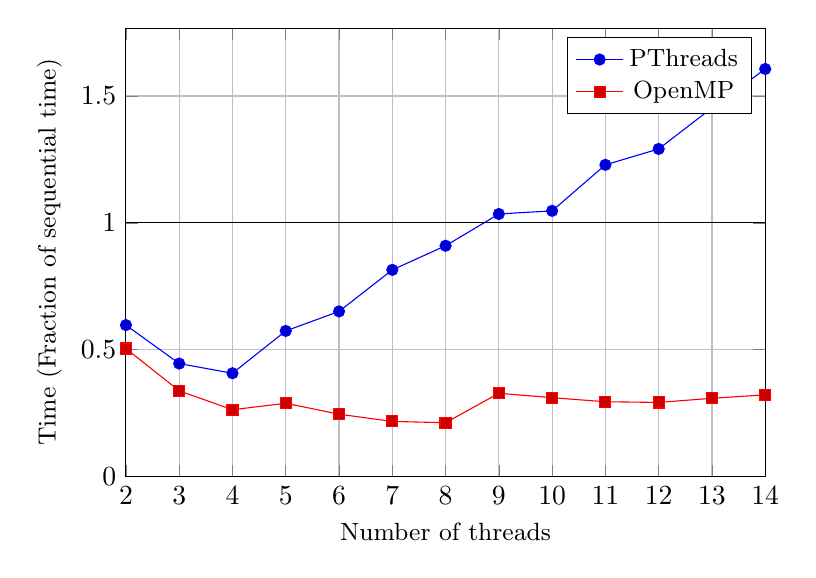
\begin{tikzpicture}
    \begin{axis}[
        width=0.8\textwidth,
        height=0.6\textwidth,
        xtick={2,...,14},
        xmin=2,
        xmax=14,
        ymin=0,
        grid=both,
        legend entries={\small PThreads,\small OpenMP},
        xlabel={\small Number of threads},
        ylabel={\small Time (Fraction of sequential time)}
      ]
      \addplot coordinates{
        (2,0.596941)
        (3,0.445256)
        (4,0.407209)
        (5,0.573977)
        (6,0.650869)
        (7,0.814665)
        (8,0.909659)
        (9,1.0349)
        (10,1.04726)
        (11,1.22862)
        (12,1.29125)
        (13,1.45297)
        (14,1.60644)};
      \addplot coordinates{
        (2,0.504375)
        (3,0.337991)
        (4,0.263352)
        (5,0.288928)
        (6,0.245644)
        (7,0.217354)
        (8,0.21215)
        (9,0.328347)
        (10,0.310834)
        (11,0.294817)
        (12,0.292123)
        (13,0.308487)
        (14,0.322058)};
      \draw (axis cs:2,1) -- (axis cs:14,1);
    \end{axis}
  \end{tikzpicture}
\end{center}
\section{System specification}
The CPU of the system used for the plot data was an Intel i7 2600k running at the frequency of 4GHz. The system was able to use 4 cores with Hyper-threading enabled, meaning the possible to use 8 logical cores simultaneously with the drawback that the performance gain from using more than 4 cores varies depending on the tasks.
\section{Questions}
\begin{enumerate}[label=\Alph*.]
\item \textbf{What kind of parallelism is exposed in the identified method?}\\
  
\item \textbf{How is the workload distributed across the threads?}\\
  
\item \textbf{Which number of thread gives you the best results? Why?}\\
  4 or 8 threads gives the best results depending on which implementation that was used. OpenMP gives the best performance at 8 threads while the PThreads implementation at 4 threads. ??????? Our conclusion is that the overhead from PThreads counter the performance gain from the Hyper-threading and makes it lose performance.
\item \textbf{Which version (OpenMP, Pthreads) gives you better results? Why?}\\
  
\end{enumerate}
\section{How to run}
The demo will be runned with a gui and using the serial implementation if no flag has overwritten the settings. The following flags can be used to alter the demo and change the implementation for the tick function.
\begin{itemize}[label=,leftmargin=0pt]
\item \textbf{-\--timing-mode} - Without gui.
\item \textbf{-\--pthread} - With PThreads implementation.
\item \textbf{-\--omp} - With OpenMP implementation.
\item \textbf{-\--silent} - Won't print anything.
\item \textbf{-\--plot} - Store the timing to the end of the file testdata.txt
\end{enumerate}
\end{document}
